%
% $Id: chapterFive.tex
%

% A first, optional argument in [ ] is the title as displayed in the table of contents
% The second argument is the title as displayed here.  Use \\ as appropriate in
%   this title to get desired line breaks

%----------------------------------------------------------------------------------------
% GPU
%----------------------------------------------------------------------------------------
\chapter[Parallel processing]{Parallel processing}
\label{chp:gpu}

A description of a new method, known as CWM, which produces an approximate solution to Riemann problems of ideal MHD that contain only regular waves without knowledge of the exact solution  was completed in the last chapter.  The final chapter of this dissertation describes the implementation of a multidimensional flow solver for HD and MHD capable of shared memory parallelism on both a CPU and GPU.  An overview of the multidimensional algorithms and grid structure is given.  Although the HD solver is relatively unchanged, CT \citep{Evans:1988} is incorporated into the MHD solver to ensure that $\divergebf{B} = 0$ throughout the simulation (assuming it was initially zero).  Important concepts for parallel programming on shared memory devices, e.g., avoiding memory contention, are described.  A performance comparison of parallel execution for three multidimensional test problems of HD and MHD is given.  We find a performance increase of seven times for the GPU over the CPU when measured by cells per second.  

%----------------------------------------------------------------------------------------
%	2D Algorithms
%----------------------------------------------------------------------------------------
\section[Methods for ideal MHD in higher dimensions]{Methods for ideal MHD in higher dimensions}          
\label{sec:2d_mhd}

Care must be taken in multidimensional MHD simulations to ensure errors associated with \divergebf{B} do not grow large enough to introduce numerical instabilities.  A number of different approaches have been devised to contain the growth of \divergebf{B}.  A brief description of a few of the more popular approaches is given below.  For a thorough review and a performance comparison of the schemes discussed below, see \citep{Toth:2000}.  

\citet{Powell:1999} derived the following non-conservative form of \eqref{eqn:mhd1} - \eqref{eqn:mhd4} where source terms proportional to \divergebf{B} are added to the right-hand side
\begin{gather}
\label{eqn:8wave1} \pd{\rho}{t} + \diverge{\left(\rho\mbf{v}\right)} = 0 \text{ ,} \\
\label{eqn:8wave2} \pd{(\rho \mbf{v})}{t} + \diverge{\left[ \outerproduct{\rho\mbf{v}}{\mbf{v}} + \left( p_g + \frac{B^2}{2}\right)\underline{\mbf{I}} - \outerproductbf{B}{B}\right]}  = -\mathbf{B}(\divergebf{B}) \text{ ,}\\
\label{eqn:8wave3} \pd{E}{t} + \diverge{\left[ \left(E + p_g + \frac{B^2}{2}\right)\mbf{v} - \innerproduct{\mbf{v}}{\outerproductbf{B}{B}}\right]}  = -\mathbf{v}\cdot\mathbf{B}(\divergebf{B}) \text{ , and} \\
\label{eqn:8wave4} \pdbf{B}{t} + \diverge{\left[ \outerproductbf{v}{B} - \outerproductbf{B}{v}\right]}  = -\mathbf{v}(\divergebf{B}) \text{.}
\end{gather}
It is known as the eight-wave scheme with the eighth wave corresponding to the propagation of \divergebf{B}.  

\citet{Brackbill:1980} introduced a corrective step for $\mbf{B}$ where the updated solution is projected to one that is  divergence free.  The so-called projection scheme corrects the updated magnetic field by subtracting the scalar potential associated with the updated field.  This is done by writing the updated solution $\mbf{B}^*$ as the sum of the curl and gradient of the vector and scalar potentials,
\begin{gather}
\label{eqn:projection1}
\mbf{B}^* = \curlbf{A} + \grad{\phi}.
\end{gather}
The correction of \eqref{eqn:projection1} is found by taking the curl of both sides and solving the resulting Poisson equation
\begin{gather}
\label{eqn:projection_poisson}
\laplace{\phi} = \diverge{\mbf{B}^*}.
\end{gather} 
The solution of \eqref{eqn:projection_poisson} is then subtracted from $\mbf{B}^*$ to give the time advanced magnetic field as
\begin{gather}
\label{eqn:projection2}
\mbf{B}^{n+1} = \mbf{B}^* - \grad{\phi}.
\end{gather} 
In order for $\diverge{\mbf{B}^{n+1}} = 0$, the Laplacian of \eqref{eqn:projection_poisson} must be calculated as the divergence of the gradient.

%-----------------------------------------------------------------
% CT grid geometry
%-----------------------------------------------------------------
\begin{figure}[htbp]\figSpace
\begin{center}
\tikzsetnextfilename{ct_grid}
%----------------------------------------------------------------------------------------
% ct_grid.tex
%----------------------------------------------------------------------------------------

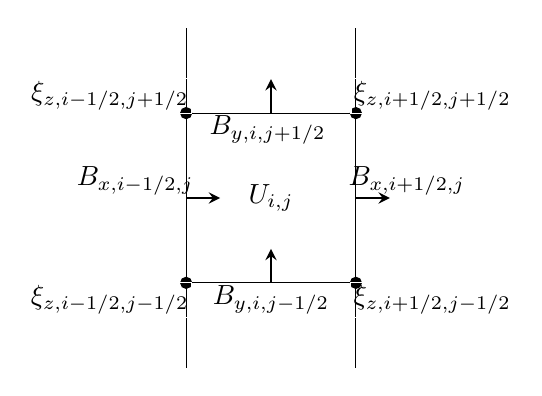
\begin{tikzpicture}[scale = {0.0125\linewidth},%inner sep = 1pt,
  >=stealth, %
  inner sep=1pt, outer sep=0pt,%
  axis/.style={thick,->},
  base node/.style={circle,draw,minimum size=4pt},
  wave/.style={thick,color=#1,smooth},
  polaroid/.style={fill=black!60!white, opacity=0.3}]

%% \draw[line width=1pt] (0.0,0.0)--(1.0,0.0);
%% \draw[line width=1pt] (0.0,0.0)--(0.0,1.0);
%% \draw[line width=1pt] (0.0,1.0)--(1.0,1.0);
%% \draw[line width=1pt] (1.0,0.0)--(1.0,1.0);

\draw[] (0.0,0.25)--(1.0,0.25);
\draw[] (0.0,0.75)--(1.0,0.75);
\draw[] (0.25,0.0)--(0.25,1.0);
\draw[] (0.75,0.0)--(0.75,1.0);

\node[draw=white] (Ucc) at (0.5,0.5) {$\mbf{U}_{i,j}$};

\draw[-stealth,thick] (0.75,0.5) -- (0.85,0.5); 
\node[] at (0.9,0.55) {$B_{x,i+1/2,j}$};

\draw[-stealth,thick] (0.25,0.5) -- (0.35,0.5); 
\node[] at (0.1,0.55) {$B_{x,i-1/2,j}$};

\draw[-stealth,thick] (0.5,0.75) -- (0.5,0.85); 
\node[] at (0.49,0.7) {$B_{y,i,j+1/2}$};

\draw[-stealth,thick] (0.5,0.25) -- (0.5,0.35); 
\node[] at (0.5,0.2) {$B_{y,i,j-1/2}$};

\node[base node,fill = black] at (0.25,0.25) {};
\node[base node,fill = black] at (0.25,0.75) {};
\node[base node,fill = black] at (0.75,0.25) {};
\node[base node,fill = black] at (0.75,0.75) {};

\node[draw=white] (ez1) at (0.025,0.2) {$\xi_{z,i-1/2,j-1/2}$};
\node[draw=white] (ez2) at (0.975,0.2) {$\xi_{z,i+1/2,j-1/2}$};
\node[draw=white] (ez3) at (0.025,0.8) {$\xi_{z,i-1/2,j+1/2}$};
\node[draw=white] (ez4) at (0.975,0.8) {$\xi_{z,i+1/2,j+1/2}$};

%% \draw[-line width=1pt] (0,0.7)--(0,0.75);  
%% \draw[line width=1pt] (-0,0)--(-0.75,0);
%% \node[draw=white] (sr) at (0.58457,0.33750) {$S_r$};
%% \node[draw=white] (ssr) at (0.33750,0.58457) {$S^*_r$};
%% \node[draw=white] (cd) at (0.058830,0.67243) {$S_m$};
%% \node[draw=white] (ssl) at (-0.33750,0.58457) {$S^*_l$};
%% \node[draw=white] (sl) at (-0.58457,0.33750) {$S_l$};

%% \node[draw=white] (ur) at (0.43467,0.11647) {$\mbf{U}_{r}$};
%% \node[draw=white] (usl) at (0.31820,0.31820) {$\mbf{U}^*_{r}$};
%% \node[draw=white] (usr) at (0.11647,0.43467) {$\mbf{U}^*_{2r}$};
%% \node[draw=white] (usr) at (-0.11647,0.43467) {$\mbf{U}^*_{2l}$};
%% \node[draw=white] (usl) at (-0.31820,0.31820) {$\mbf{U}^*_{l}$};
%% \node[draw=white] (ul) at (-0.43467,0.11647) {$\mbf{U}_{l}$};

%% \draw (0,0) -- (sr);  
%% \draw (0,0) -- (ssr);  
%% \draw (0,0) -- (cd);  
%% \draw (0,0) -- (ssl);  
%% \draw (0,0) -- (sl);  

\end{tikzpicture}

\end{center}
\caption{Staggered field geometry of the constrained transport scheme.  The components of the magnetic field are located at the cell interfaces, and $\xi_z$ is located at the cell corners.}
\label{fig:ct_grid}
\figSpace
\end{figure}

The final approach discussed here, and the one implemented for this dissertation, is the CT method of \citet{Evans:1988}.  For CT, the $\divergebf{B} = 0$ is maintained by staggering the grid with the magnetic field components placed at the cell interfaces.  The electromotive force $\mbf{E} = -\crossproductbf{v}{B}$ is defined along the edges in three-dimensions and at the cell corners in two-dimensions.  Following the notation of \citep{Stone:2008}, the z-component of the electromotive force is denoted $\xi_z$.  The placement of $\mbf{B}$ and $\xi_z$ in two-dimensions is shown in Figure~\ref{fig:ct_grid}, with $B_x$ placed at $x_{i+1/2}, y_j$ and $B_y$ place at $x_i,y_{j+1/2}$.  The integration is done along cell edges in terms of finite areas instead of finite volumes.  The updated magnetic field components are
\begin{gather}
B^{n+1}_{x,i+1/2,j} = B^{n}_{x,i+1/2,j} - \frac{\delta t}{\delta y}\left( \xi_{z,i+1/2,j+1/2} - \xi_{z,i+1/2,j-1/2}\right), \text{ and} \\
B^{n+1}_{y,i,j+1/2} = B^{n}_{y,i,j+1/2} + \frac{\delta t}{\delta x}\left( \xi_{z,i+1/2,j+1/2} - \xi_{z,i-1/2,j-1/2}\right).
\end{gather}
Due to perfect cancellation, the numerical divergence in the cell 
\begin{gather}
(\diverge{\mbf{B}})_{i,j} = \frac{1}{\delta x} \left( B_{x,i+1/2,j}  - B_{x,i-1/2,j}\right) + \frac{1}{\delta y} \left( B_{y,i,j+1/2}  - B_{y,i,j-1/2}\right) 
\end{gather}
remains zero after the solution is updated.

The \glspl{emf} are initially calculated at the faces and must be integrated to the corners.  \citet{Gardiner:2005} argued that simple averaging across the faces will produce incorrect results for plane-parallel grid-aligned flows and proposed an upwind method.  They gave the EMFs at the cell corners as 
\begin{gather}
\xi_{z,i+1/2,j+1/2} = \frac{1}{4}(\xi_{z,i+1/2,j} + \xi_{z,i+1/2,j+1} + \xi_{z,i,j+1/2} + \xi_{z,i+1,j+1/2}) \\
\;\;\;\;\;\;\;\;\;\;\;\;  +  \frac{\delta y}{8} \left( \left(\pd{\xi_z}{y}\right)_{i+1/2,j+1/4} - \left(\pd{\xi_z}{y}\right)_{i+1/2,j+3/4} \right) \\
\;\;\;\;\;\;\;\;\;\;\;\;  +  \frac{\delta x}{8} \left( \left(\pd{\xi_z}{x}\right)_{i+1/4,j+1/2} - \left(\pd{\xi_z}{y}\right)_{i+3/4,j+1/2} \right) .
\end{gather}  

The derivatives of the EMF, $\partial \xi_z / \partial y$ ($\partial \xi_z / \partial x$) , at the x (y) interfaces are upwinded based on the contact mode.  In \citep{Gardiner:2005}, they are given as
\begin{gather}
\label{eqn:emf_upwind}
\left( \pd{\xi_z}{y}\right)_{i+1/2,j+1/4} =
\begin{cases}
\left( \pd{\xi_z}{y}\right)_{i,j+1/4} & \text{if}\;\;\; v_{n,i-+1/2,j} > 0 , \\
\left( \pd{\xi_z}{y}\right)_{i+1,j+1/4} & \text{if}\;\;\; v_{n,i+1/2,j} < 0 , \\
\frac{1}{2}\left(\left( \pd{\xi_z}{y}\right)_{i,j+1/4} + \left( \pd{\xi_z}{y}\right)_{i+1,j+1/4} \right)& \text{otherwise}.
\end{cases}
\end{gather}
The derivatives are 
\begin{gather}
\left( \pd{\xi_z}{y} \right)_{i,j-1/4} = \frac{\xi^r_{z,i,j} - \xi_{z,i,j-1/2}}{2\delta y}.
\end{gather}
where $\xi^r_{z,i,j}$ is a reference EMF computed at the cell center, see Figure 5 of \citep{Stone:2008}.  Similar expressions can be obtained for $\partial \xi_z / \partial x$. 

The steps of the two-dimensional algorithm are given as follows:
\begin{enumerate}
\item Calculate the fluxes at each interface replacing the normal component of the magnetic field at cell center with the value at the interface.
\item Calculate the EMFs at the cell corners using the algorithm described above.
\item Calculate the reference field $\xi^r_{i,j}$ at the cell centers.
\item Update the hydrodynamical conserved variables and $B_z$ at the cell centers.
\item Update the magnetic field at each interface using CT.
\item Calculate the normal and tangential components of the cell-centered magnetic field as the average of the interface values.
\item Advance the solution in time.
\item Apply higher order extension.
\item Update the solution.
\item Calculate new time step and repeat steps 1-9 until stopping criteria is met.
\end{enumerate}

In the next section, a detailed description is given of the parallel implementations of the one- and two-dimensional algorithms of this dissertation.

%----------------------------------------------------------------------------------------
%	Shared Memory Parallelism
%----------------------------------------------------------------------------------------
\section[Shared memory parallelism]{Shared memory parallelism}
\label{sec:shared_memory}

Shared memory parallelism refers to simultaneous execution on a common section of memory.  It was implemented for this dissertations using Thrust, a \cpp$\,$  parallel template library based on the \gls{stl}.  It supports four device backends: \gls{cuda}, \gls{omp}, \gls{tbb}, and the standard \cpp$\,$  device for serial runs.  The CUDA backend utilizes the GPU, while the OMP and TBB backends utilize multi-core processing on the CPU.  This dissertation compares the performance of the the CUDA and OMP backends.

It is essential that there is no overlap of memory access of the different threads.  In fluid dynamics, this is achieved by \emph{coloring} the faces/edges.  Coloring refers to grouping the faces/edges, i.e., coloring them, so that no two members of the group need to access the same memory space for the calculations.  For FV schemes, an iteration over the faces in serial becomes an iteration over the colors and the corresponding faces in parallel. 

%-----------------------------------------------------------------
% Face coloring 1
%-----------------------------------------------------------------
\begin{figure}[htbp]\figSpace
\begin{center}
\tikzsetnextfilename{face_color_1}
%----------------------------------------------------------------------------------------
% face_color_1.tex
%----------------------------------------------------------------------------------------

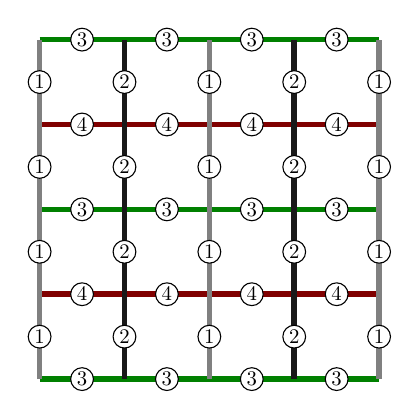
\begin{tikzpicture}[scale = {0.0125\linewidth},
  >=stealth, %
  inner sep=1pt, outer sep=0pt,%
  axis/.style={thick,->},
  base node/.style={circle,draw,minimum size=5pt},
  wave/.style={thick,color=#1,smooth},
  polaroid/.style={fill=black!60!white, opacity=0.3}]


\draw[green!50!black,line width=2pt] (0.0,0.0)--(0.25,0.0);
\draw[green!50!black,line width=2pt] (0.25,0.0)--(0.5,0.0);
\draw[green!50!black,line width=2pt] (0.5,0.0)--(0.75,0.0);
\draw[green!50!black,line width=2pt] (0.75,0.0)--(1.0,0.0);

\draw[red!50!black,line width=2pt] (0.0,0.25)--(0.25,0.25);
\draw[red!50!black,line width=2pt] (0.25,0.25)--(0.5,0.25);
\draw[red!50!black,line width=2pt] (0.5,0.25)--(0.75,0.25);
\draw[red!50!black,line width=2pt] (0.75,0.25)--(1.0,0.25);

\draw[green!50!black,line width=2pt] (0.0,0.5)--(0.25,0.5);
\draw[green!50!black,line width=2pt] (0.25,0.5)--(0.5,0.5);
\draw[green!50!black,line width=2pt] (0.5,0.5)--(0.75,0.5);
\draw[green!50!black,line width=2pt] (0.75,0.5)--(1.0,0.5);

\draw[red!50!black,line width=2pt] (0.0,0.75)--(0.25,0.75);
\draw[red!50!black,line width=2pt] (0.25,0.75)--(0.5,0.75);
\draw[red!50!black,line width=2pt] (0.5,0.75)--(0.75,0.75);
\draw[red!50!black,line width=2pt] (0.75,0.75)--(1.0,0.75);

\draw[green!50!black,line width=2pt] (0.0,1.0)--(0.25,1.0);
\draw[green!50!black,line width=2pt] (0.25,1.0)--(0.5,1.0);
\draw[green!50!black,line width=2pt] (0.5,1.0)--(0.75,1.0);
\draw[green!50!black,line width=2pt] (0.75,1.0)--(1.0,1.0);

\draw[black!50!,line width=2pt] (0.0,0.0)--(0.0,0.25);
\draw[black!50!,line width=2pt] (0.0,0.25)--(0.0,0.5);
\draw[black!50!,line width=2pt] (0.0,0.5)--(0.0,0.75);
\draw[black!50!,line width=2pt] (0.0,0.75)--(0.0,1.0);

\draw[black!90!,line width=2pt] (0.25,0.0)--(0.25,0.25);
\draw[black!90!,line width=2pt] (0.25,0.25)--(0.25,0.5);
\draw[black!90!,line width=2pt] (0.25,0.5)--(0.25,0.75);
\draw[black!90!,line width=2pt] (0.25,0.75)--(0.25,1.0);

\draw[black!50!,line width=2pt] (0.5,0.0)--(0.5,0.25);
\draw[black!50!,line width=2pt] (0.5,0.25)--(0.5,0.5);
\draw[black!50!,line width=2pt] (0.5,0.5)--(0.5,0.75);
\draw[black!50!,line width=2pt] (0.5,0.75)--(0.5,1.0);

\draw[black!90!,line width=2pt] (0.75,0.0)--(0.75,0.25);
\draw[black!90!,line width=2pt] (0.75,0.25)--(0.75,0.5);
\draw[black!90!,line width=2pt] (0.75,0.5)--(0.75,0.75);
\draw[black!90!,line width=2pt] (0.75,0.75)--(0.75,1.0);

\draw[black!50!,line width=2pt] (1.0,0.0)--(1.0,0.25);
\draw[black!50!,line width=2pt] (1.0,0.25)--(1.0,0.5);
\draw[black!50!,line width=2pt] (1.0,0.5)--(1.0,0.75);
\draw[black!50!,line width=2pt] (1.0,0.75)--(1.0,1.0);

\begin{scope}[every node/.style={scale=.75}]

\node[base node,fill = white] at (0.0,0.125) {$1$};
\node[base node,fill = white] at (0.0,0.375) {$1$};
\node[base node,fill = white] at (0.0,0.625) {$1$};
\node[base node,fill = white] at (0.0,0.875) {$1$};

\node[base node,fill = white] at (0.25,0.125) {$2$};
\node[base node,fill = white] at (0.25,0.375) {$2$};
\node[base node,fill = white] at (0.25,0.625) {$2$};
\node[base node,fill = white] at (0.25,0.875) {$2$};

\node[base node,fill = white] at (0.5,0.125) {$1$};
\node[base node,fill = white] at (0.5,0.375) {$1$};
\node[base node,fill = white] at (0.5,0.625) {$1$};
\node[base node,fill = white] at (0.5,0.875) {$1$};

\node[base node,fill = white] at (0.75,0.125) {$2$};
\node[base node,fill = white] at (0.75,0.375) {$2$};
\node[base node,fill = white] at (0.75,0.625) {$2$};
\node[base node,fill = white] at (0.75,0.875) {$2$};

\node[base node,fill = white] at (1.0,0.125) {$1$};
\node[base node,fill = white] at (1.0,0.375) {$1$};
\node[base node,fill = white] at (1.0,0.625) {$1$};
\node[base node,fill = white] at (1.0,0.875) {$1$};

\node[base node,fill = white] at (0.125,0.0) {$3$};
\node[base node,fill = white] at (0.375,0.0) {$3$};
\node[base node,fill = white] at (0.625,0.0) {$3$};
\node[base node,fill = white] at (0.875,0.0) {$3$};

\node[base node,fill = white] at (0.125,0.25) {$4$};
\node[base node,fill = white] at (0.375,0.25) {$4$};
\node[base node,fill = white] at (0.625,0.25) {$4$};
\node[base node,fill = white] at (0.875,0.25) {$4$};

\node[base node,fill = white] at (0.125,0.5) {$3$};
\node[base node,fill = white] at (0.375,0.5) {$3$};
\node[base node,fill = white] at (0.625,0.5) {$3$};
\node[base node,fill = white] at (0.875,0.5) {$3$};

\node[base node,fill = white] at (0.125,0.75) {$4$};
\node[base node,fill = white] at (0.375,0.75) {$4$};
\node[base node,fill = white] at (0.625,0.75) {$4$};
\node[base node,fill = white] at (0.875,0.75) {$4$};

\node[base node,fill = white] at (0.125,1.0) {$3$};
\node[base node,fill = white] at (0.375,1.0) {$3$};
\node[base node,fill = white] at (0.625,1.0) {$3$};
\node[base node,fill = white] at (0.875,1.0) {$3$};

\end{scope}


\end{tikzpicture}

\end{center}
\caption{Colored grouping of interior faces for avoiding memory contention with cell centered finite volume schemes.  Four groups, labeled 1-4, are required.}
\label{fig:face_color_1}
\figSpace
\end{figure}

A possible coloring, and the one implemented for this dissertation, of the interior faces for cell-centered FV schemes is shown in Figure~\ref{fig:face_color_1}.  For each loop, the flux at the face is calculated and the residual at the cells is built by adding the contribution of each face.  Coloring ensures two faces will not attempt to update the residual of a cell simultaneously.

%-----------------------------------------------------------------
% Face coloring 2
%-----------------------------------------------------------------
\begin{figure}[htbp]\figSpace
\begin{center}
\tikzsetnextfilename{face_color_2}
%----------------------------------------------------------------------------------------
% face_color_2.tex
%----------------------------------------------------------------------------------------

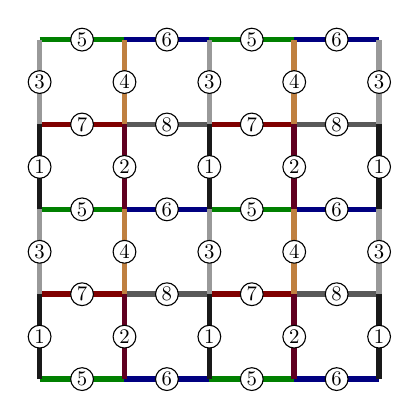
\begin{tikzpicture}[scale = {0.0125\linewidth},
  >=stealth, %
  inner sep=1pt, outer sep=0pt,%
  axis/.style={thick,->},
  base node/.style={circle,draw,minimum size=1pt},
  wave/.style={thick,color=#1,smooth},
  polaroid/.style={fill=black!60!white, opacity=0.3}]


\draw[green!50!black,line width=2pt] (0.0,0.0)--(0.25,0.0);
%% \node[mark size= 4pt ] at (0.09,0.0) {\pgfuseplotmark{*}};
\draw[blue!50!black,line width=2pt] (0.25,0.0)--(0.5,0.0);
\draw[green!50!black,line width=2pt] (0.5,0.0)--(0.75,0.0);
%% \node[mark size= 4pt ] at (0.34,0.0) {\pgfuseplotmark{square*}};
\draw[blue!50!black,line width=2pt] (0.75,0.0)--(1.0,0.0);

\draw[red!50!black,line width=2pt] (0.0,0.25)--(0.25,0.25);
%% \node[mark size= 4pt ] at (0.34,0.25) {\pgfuseplotmark{square*}};
\draw[black!65!,line width=2pt] (0.25,0.25)--(0.5,0.25);
\draw[red!50!black,line width=2pt] (0.5,0.25)--(0.75,0.25);
\draw[black!65!,line width=2pt] (0.75,0.25)--(1.0,0.25);

\draw[green!50!black,line width=2pt] (0.0,0.5)--(0.25,0.5);
\draw[blue!50!black,line width=2pt] (0.25,0.5)--(0.5,0.5);
\draw[green!50!black,line width=2pt] (0.5,0.5)--(0.75,0.5);
\draw[blue!50!black,line width=2pt] (0.75,0.5)--(1.0,0.5);

\draw[red!50!black,line width=2pt] (0.0,0.75)--(0.25,0.75);
\draw[black!65!,line width=2pt] (0.25,0.75)--(0.5,0.75);
\draw[red!50!black,line width=2pt] (0.5,0.75)--(0.75,0.75);
\draw[black!65!,line width=2pt] (0.75,0.75)--(1.0,0.75);

\draw[green!50!black,line width=2pt] (0.0,1.0)--(0.25,1.0);
\draw[blue!50!black,line width=2pt] (0.25,1.0)--(0.5,1.0);
\draw[green!50!black,line width=2pt] (0.5,1.0)--(0.75,1.0);
\draw[blue!50!black,line width=2pt] (0.75,1.0)--(1.0,1.0);

\draw[black!90!,line width=2pt] (0.0,0.0)--(0.0,0.25);
\draw[black!40!,line width=2pt] (0.0,0.25)--(0.0,0.5);
\draw[black!90!,line width=2pt] (0.0,0.5)--(0.0,0.75);
\draw[black!40!,line width=2pt] (0.0,0.75)--(0.0,1.0);

\draw[purple!50!black,line width=2pt] (0.25,0.0)--(0.25,0.25);
\draw[brown,line width=2pt] (0.25,0.25)--(0.25,0.5);
\draw[purple!50!black,line width=2pt] (0.25,0.5)--(0.25,0.75);
\draw[brown,line width=2pt] (0.25,0.75)--(0.25,1.0);

\draw[black!90!,line width=2pt] (0.5,0.0)--(0.5,0.25);
\draw[black!40!,line width=2pt] (0.5,0.25)--(0.5,0.5);
\draw[black!90!,line width=2pt] (0.5,0.5)--(0.5,0.75);
\draw[black!40!,line width=2pt] (0.5,0.75)--(0.5,1.0);

\draw[purple!50!black,line width=2pt] (0.75,0.0)--(0.75,0.25);
\draw[brown,line width=2pt] (0.75,0.25)--(0.75,0.5);
\draw[purple!50!black,line width=2pt] (0.75,0.5)--(0.75,0.75);
\draw[brown,line width=2pt] (0.75,0.75)--(0.75,1.0);

\draw[black!90!,line width=2pt] (1.0,0.0)--(1.0,0.25);
\draw[black!40!,line width=2pt] (1.0,0.25)--(1.0,0.5);
\draw[black!90!,line width=2pt] (1.0,0.5)--(1.0,0.75);
\draw[black!40!,line width=2pt] (1.0,0.75)--(1.0,1.0);

\begin{scope}[every node/.style={scale=.75}]

\node[base node,fill = white] at (0.0,0.125) {$1$};
\node[base node,fill = white] at (0.0,0.375) {$3$};
\node[base node,fill = white] at (0.0,0.625) {$1$};
\node[base node,fill = white] at (0.0,0.875) {$3$};

\node[base node,fill = white] at (0.25,0.125) {$2$};
\node[base node,fill = white] at (0.25,0.375) {$4$};
\node[base node,fill = white] at (0.25,0.625) {$2$};
\node[base node,fill = white] at (0.25,0.875) {$4$};

\node[base node,fill = white] at (0.5,0.125) {$1$};
\node[base node,fill = white] at (0.5,0.375) {$3$};
\node[base node,fill = white] at (0.5,0.625) {$1$};
\node[base node,fill = white] at (0.5,0.875) {$3$};

\node[base node,fill = white] at (0.75,0.125) {$2$};
\node[base node,fill = white] at (0.75,0.375) {$4$};
\node[base node,fill = white] at (0.75,0.625) {$2$};
\node[base node,fill = white] at (0.75,0.875) {$4$};

\node[base node,fill = white] at (1.0,0.125) {$1$};
\node[base node,fill = white] at (1.0,0.375) {$3$};
\node[base node,fill = white] at (1.0,0.625) {$1$};
\node[base node,fill = white] at (1.0,0.875) {$3$};

\node[base node,fill = white] at (0.125,0.0) {$5$};
\node[base node,fill = white] at (0.375,0.0) {$6$};
\node[base node,fill = white] at (0.625,0.0) {$5$};
\node[base node,fill = white] at (0.875,0.0) {$6$};

\node[base node,fill = white] at (0.125,0.25) {$7$};
\node[base node,fill = white] at (0.375,0.25) {$8$};
\node[base node,fill = white] at (0.625,0.25) {$7$};
\node[base node,fill = white] at (0.875,0.25) {$8$};

\node[base node,fill = white] at (0.125,0.5) {$5$};
\node[base node,fill = white] at (0.375,0.5) {$6$};
\node[base node,fill = white] at (0.625,0.5) {$5$};
\node[base node,fill = white] at (0.875,0.5) {$6$};

\node[base node,fill = white] at (0.125,0.75) {$7$};
\node[base node,fill = white] at (0.375,0.75) {$8$};
\node[base node,fill = white] at (0.625,0.75) {$7$};
\node[base node,fill = white] at (0.875,0.75) {$8$};

\node[base node,fill = white] at (0.125,1.0) {$5$};
\node[base node,fill = white] at (0.375,1.0) {$6$};
\node[base node,fill = white] at (0.625,1.0) {$5$};
\node[base node,fill = white] at (0.875,1.0) {$6$};

\end{scope}

%% \node[base node,fill = black] at (0.0,0.25) {};
%% \node[base node,fill = black] at (0.0,0.5) {};
%% \node[base node,fill = black] at (0.0,0.75) {};
%% \node[base node,fill = black] at (0.0,1.0) {};

%% \node[base node,fill = black] at (0.25,0.0) {};
%% \node[base node,fill = black] at (0.25,0.25) {};
%% \node[base node,fill = black] at (0.25,0.5) {};
%% \node[base node,fill = black] at (0.25,0.75) {};
%% \node[base node,fill = black] at (0.25,1.0) {};

%% \node[base node,fill = black] at (0.5,0.0) {};
%% \node[base node,fill = black] at (0.5,0.25) {};
%% \node[base node,fill = black] at (0.5,0.5) {};
%% \node[base node,fill = black] at (0.5,0.75) {};
%% \node[base node,fill = black] at (0.5,1.0) {};

%% \node[base node,fill = black] at (0.75,0.0) {};
%% \node[base node,fill = black] at (0.75,0.25) {};
%% \node[base node,fill = black] at (0.75,0.5) {};
%% \node[base node,fill = black] at (0.75,0.75) {};
%% \node[base node,fill = black] at (0.75,1.0) {};

%% \node[base node,fill = black] at (1.0,0.0) {};
%% \node[base node,fill = black] at (1.0,0.25) {};
%% \node[base node,fill = black] at (1.0,0.5) {};
%% \node[base node,fill = black] at (1.0,0.75) {};
%% \node[base node,fill = black] at (1.0,1.0) {};

\end{tikzpicture}

\end{center}
\caption{Colored grouping of interior faces for avoiding memory contention with cell centered finite volume schemes plus constrained transport.  Eight groups, labeled 1-8, are required.}
\label{fig:face_color_2}
\figSpace
\end{figure}

Coloring is more complicated when CT is used in conjunction with a cell-centered FV scheme.  In this case, each loop over the faces consists of a contribution to the residual at the cell center and a contribution to the EMF at the cell corner.  Not only accessing the same cell, but also the same point must be avoided.  The coloring scheme shown in Figure~\ref{fig:face_color_1} only avoids one of these potential pitfalls, because the faces/edges of each group can access the same point simultaneously.  An alternative coloring scheme is shown in Figure~\ref{fig:face_color_2} where eight colors are used instead of four.  In this case, the faces and the edges are colored.  This is equivalent to doubling the amount of colors for the faces since edges and faces are the same in two-dimensions.

%----------------------------------------------------------------------------------------
%	GPU efficient algorithms
%----------------------------------------------------------------------------------------
\section[Efficient algorithms]{Efficient algorithms}
\label{sec:efficient_algo}

This section discusses increasing parallel performance with efficient data storage and proper utilization of computational power.  Two types of data storage are AoS and SoA.  With limited memory available on the GPU, it is important to limit data storage.  This is achieved through function composition, or operator fusion.

The goal of operator fusion is to reduce storage of temporary data for similar operations.  As an example, consider the two transformations, $f(x)$ and $g(f(x))$ \citep{Thrust}.
\begin{lstlisting}
  thrust::device_vector<float> x(n);  // independent variable
  thrust::device_vector<float> y(n);  // y = f(x)
  thrust::device_vector<float> z(n);  // z = g(y)

  // compute y = f(x)
  thrust::transform(x.begin(),x.end(),y.begin(),f());

  // compute z = g(y) 
  thrust::transform(y.begin(),y.end(),z.begin(),g());
\end{lstlisting} 
The above example requires storage of $3n$ floats, $2n$ reads, $2n$ writes, and uses $n$ temporary floats.  The operations can be fused by using transform iterators.
\begin{lstlisting}
  thrust::device_vector<float> x(n);  // independent variable
  thrust::device_vector<float> z(n);  // z = g(y) = g(f(x))

  // compute z = g(f(x))
  thrust::transform(make_transform_iterator(x.begin(),f()),
                    make_transform_iterator(x.end(),f()),
                    z.begin(),
                    g());
\end{lstlisting} 
Using \verb+transform_iterators+ reduces the storage requirements to $2n$ floats, $n$ reads, $n$ writes, and no temporary storage.  As another example, consider initializing the cell-centered variables for an HD shock tube problem in one-dimension.  The initial discontinuity is given by \verb+discontinuity_position+ and the initial left and right states are given in primitive variables by the tuples of floats \verb+state_l+ and \verb+state_r+ respectively.  The inefficient method for initializing the cell centers with conservative state variables is given below.
\begin{lstlisting}
  // type definitions
  typedef thrust::device_vector<float,float>       Point; // (x,y)
  typedef thrust::device_vector<float,float,float> Vector;// (d, mx, E)
  typedef thrust::device_vector<Point>             PointArray;  // SoA
  typedef thrust::device_vector<Vector>            VectorArray; // SoA

  int         n;                     // number of cells
  float       discontinuity_postion;
  PointArray  cell_positions(n);
  VectorArray primitive_states(ncell);
  VectorArray conservative_states(n);

  // compute cell positions 
  thrust::transform_n(thrust::make_counting_iterator(0),
                      n,
                      cell_positions.begin(),
                      cells_initialize());
  			  
  
  // set state of cell based on position                 
  thrust::transform_n(cell_positions.begin(),
                      cell_positions.size(),
                      primitive_states.begin(),
                      shock_tube_initialize(discontinuity_postion,
                                            state_l,
                                            state_r));

  // convert primitive variables to conservative variables
  thrust::transform_n(primitive_states.begin(),
                      primitive_states.size(),
                      conservative_states.begin(),
                      convert_primitive_to_conservative());
\end{lstlisting}
The storage of the cell positions and primitive variables is eliminated using the \\ \verb+make_transform_iterator+ as follows 
\begin{lstlisting}
  // type definitions
  typedef thrust::device_vector<float,float,float> Vector;// (d, mx, E)
  typedef thrust::device_vector<Vector>            VectorArray; // SoA

  int n;
  float discontinuity_postion;
  VectorArray conservative_states(n);

  // set conservative state at cell center based on position
  thrust::transform_n(make_transform_iterator(
                          make_transform_iterator(
                               make_device_counting_iterator(),
                               cells_initialize()),
                          shock_tube_initialize(discontinuity_postion,
                                                state_l,
                                                state_r)),
                       ncell(),
                       conservative_states.begin(),
                       convert_primitive_to_conservative());
\end{lstlisting}
see Appendix~\ref{app:thrust_add} for the definitions of \verb+transform_n+ and \verb+make_device_counting_iterator+.  By fusing the transformations, the need to store $5n$ floats was eliminated, the number of reads and writes was reduced by $5n$, and no temporaries were stored.  The storage requirements are reduced by $10n$ in the case of multi-dimensional MHD.  Transform iterators help reduce the amount of stored data, however, it is important to properly store the remaining data to achieve memory coalescing.

Memory coalescing occurs when multiple memory addresses are accessed with a single transaction.  A warp is 32 consecutive threads on the GPU.  It can access 128 bytes, i.e., 32 single precision values, with one transaction.  If memory is uncoalesced, multiple transactions are required to load 128 bytes.  Coalescing does not occur when data is stored with AoS, it will however, with SoA.  Below is an example of a structure containing one-dimensional hydrodynamic state variables.
\begin{lstlisting}
struc conservative_variables{
  float density;
  float momentum_x;
  float energy;
}

conservative_variables *state;  // AoS

state[i].density = some_number;
state[i].momentum_x = another_number;
state[i].energy = one_more_number;
\end{lstlisting} 

To ensure memory is coalesced, the variables need to be stored in an SoA, as shown below.
\begin{lstlisting}
struc conservative_variables{
  float *density;
  float *momentum_x;
  float *energy;
}

conservative_variables state; // SoA

state.density[i] = some_number;
state.momentum_x[i] = another_number;
state.energy[i] = one_more_number;
\end{lstlisting} 
Memory coalescing can be achieved with thrust through the use of the \verb+zip_iteraor+.  It creates tuples from arrays on the fly.  Converting from primitive variables to conservative variables using the slower AoS approach is shown below.
\begin{lstlisting}
struc convert_primitive_to_conservative 
  : public thrust::unary_function<primitive_variables,
                                 conservative_variables>
{
  float _gamma;
  
  convert_primitive_to_conservative(float gamma)
  : _gamma(gamma) {}

  __host__ __device__
  conservative_variables operator()(const primitive_variables& pstate)

  float half = 1.0f/2.0f;
  float d  = pstate.density;
  float vx = pstate.velocity_x;
  float pg = pstate.pressure_gas;

  float density = d;
  float momentum_x = d*vx;
  float energy = pg/(1.0f - this->_gamma) + half*d*vx*vx;
  
  return make_conservative_variables(density,momentum_x,energy);
}

thrust::device_vector<primitive_variables>    pstate(n);  // AoS
thrust::device_vector<conservative_variables> state(n);   // AoS
thrust::transform_n(pstate.begin(),
                    pstate.size(),
                    state.begin(),
                    convert_primitive_to_conservative(gamma));
\end{lstlisting} 
The faster SoA approach using the \verb+zip_operator+ is shown below.
\begin{lstlisting} 
struc convert_primitive_to_conservative
  : public thrust::unary_function<tuple<float,float,float>,
                                  tuple<float,float,float>>
{
  float _gamma;
  
  convert_primitive_to_conservative(float gamma)
  : _gamma(gamma) {}

  __host__ __device__
  tuple<float,float,float>operator()(const tuple<float,float,float>& pstate)

  float half = 1.0f/2.0f;
  float d  = thrust::get<0>(pstate);
  float vx = thrust::get<1>(pstate);
  float pg = thrust::get<2>(pstate);

  float density = d;
  float momentum_x = d*vx;
  float energy = pg/(1.0f - this->_gamma) + half*d*vx*vx;
  
  return make_tuple(density,momentum_x,energy);
}
thrust::device_vector<float> d(n),vx(n),pg(n); 
thrust::device_vector<float> mx(n),en(n); 
thrust::transform_n(thrust::make_zip_iterator(make_tuple(d.begin(),
                                                        vx.begin(),
                                                        pg.begin())),
                    n,
                    thrust::make_zip_iterator(make_tuple(d.begin(),
                                                        mx.begin(),
                                                        en.begin())),
                    convert_primitive_to_conservative(gamma));
\end{lstlisting} 

The algorithms and techniques discussed above have been implemented in a multidimensional hydrodynamic and ideal magnetohydrodynamic solver capable of shared memory parallelism.  In the following section, the accuracy and performance of the code is demonstrated on some well known test problems, namely Kelvin-Helmholtz instability, spherical blast waves, and Orzag-Tang vortex.  

%----------------------------------------------------------------------------------------
%	Performance Results
%----------------------------------------------------------------------------------------
\section[Performance results]{Performance results}
\label{sec:gpu_results}

In Section~\ref{sec:shared_memory} performance enhancing techniques such as operator fusion and SoA data storage were described.  The algorithms described in Section~\ref{sec:2d_mhd} were implemented in an edge-based finite-volume flow solver.  The performance results on a Dell Precision 7500 workstation with a (Dual CPU) Intel Xeon E5645 @ 2.40 Ghz and a GeFroce GTX TITAN GPU with a memory bandwidth of 288.4 GB/sec and 2688 CUDA cores are given for three test cases, the Kelvin-Helmholtz instability, spherical blast waves, and Orzag-Tang vortex.  In all three tests, we use the initial conditions of \citep{url:athena} for comparison purposes.

%----------------------------------------------------------------
% KH-instability
%-----------------------------------------------------------------
\begin{figure}[htbp]\figSpace
\begin{center} 
\begin{tabular}{c}
%% 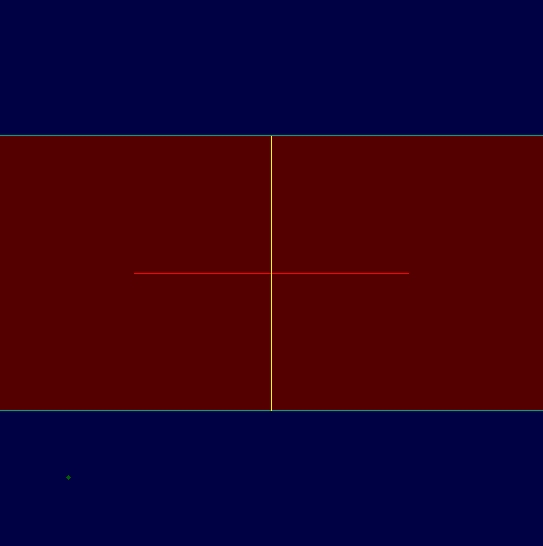
\includegraphics[width=0.25\textheight]{fig/kh0.jpg} \\ 
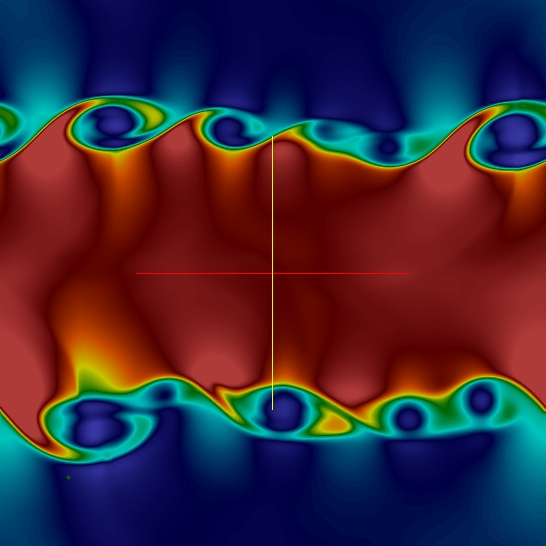
\includegraphics[width=0.4\textheight]{fig/kh1.jpg} \\ 
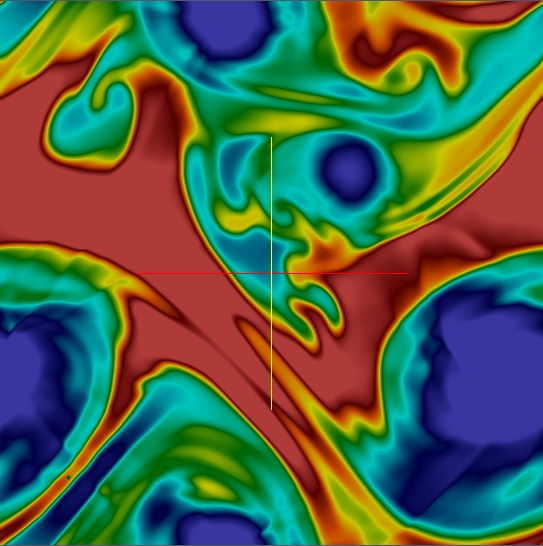
\includegraphics[width=0.4\textheight]{fig/kh5.jpg} 
\end{tabular}
\caption{The Kelvin-Helmoltz instability, $\rho$ at times: $t=1$ (top) and $t=5$ (bottom).  Simulation performed on a $400 \times 400$ grid of triangular elements with code written for this dissertation available at: \protect\gitrepo.}
\end{center} 
\label{fig:kh_instability}
\figSpace
\end{figure}

The Kelvin-Helmholtz instability \citep{hydro_stability} considers a slip surface, i.e., a discontinuity between oppositely directed flows.  The version of the test considered here is identical to the version given by \citet{url:athena}.  The simulation is performed on a square domain, $[0,1] \times [0,1]$, with periodic boundaries everywhere.  The flow speed is $0.5$; it is in the $-x$ direction for $ y < 0.25$ and $y > 0.75$, where $\rho = 1$, and in the $x$ direction for $0.25 \le y \le 0.75$, where $\rho = 2$.  The gas pressure is initially $2.5$ everywhere and the ratio of specific heats is $\gamma = 1.4$.  The instability is produced by adding random perturbations with a peak amplitude of $0.01$ to both the $x$ and $y$ velocities.  In the case of ideal MHD, the initial magnetic field is $B_x/\sqrt{4\pi} = 0.5$.

The density at times $t=1$ and $t=5$ is shown in the top and bottom panels of Figure~\ref{fig:kh_instability} respectively.  The initial conditions are shown in Figure~\ref{fig:kh_instability_ics} of Appendix~\ref{app:kh_instability_ics}.  The boundary between the two fluids is well resolved at later times.  This indicates numerical diffusion is not excessive.  If excessive numerical diffusion were present, the instability would be suppressed \citep{url:athena}. 

%----------------------------------------------------------------
% KH-instability MHD
%-----------------------------------------------------------------
\begin{figure}[htbp]\figSpace
\begin{center} 
\begin{tabular}{c}
%% 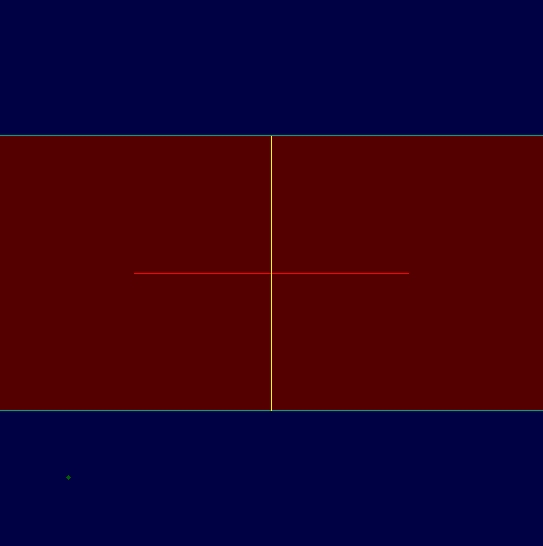
\includegraphics[width=0.25\textheight]{fig/kh0.jpg} \\ 
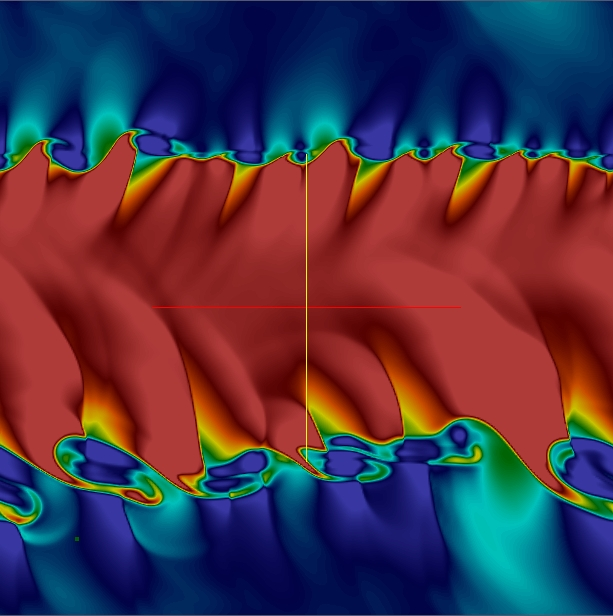
\includegraphics[width=0.4\textheight]{fig/kh_mhd_d_0275.jpg} \\ 
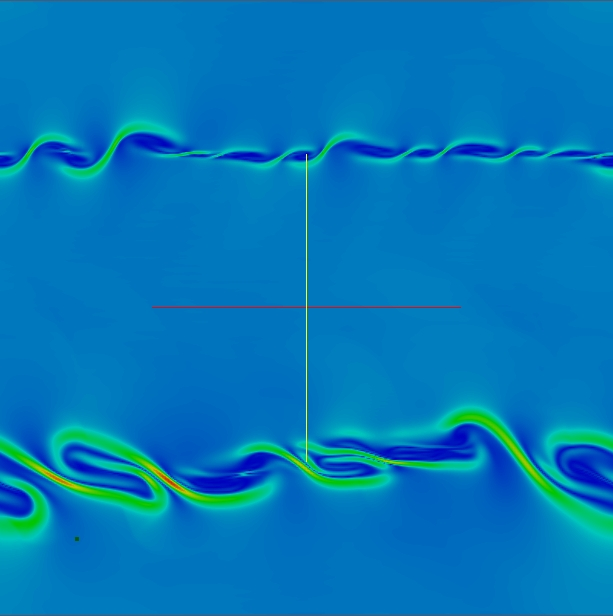
\includegraphics[width=0.4\textheight]{fig/kh_mhd_bmag_0275.jpg} 
\end{tabular}
\caption{The MHD Kelvin-Helmoltz instability, $\rho$ (top) and $|\mbf{B}|$ (bottom) at $t=2.75$.  Simulation performed on a $400 \times 400$ grid of quadrilateral elements with code written for this dissertation available at: \protect\gitrepo.}
\end{center} 
\label{fig:kh_instability_mhd}
\figSpace
\end{figure}

%----------------------------------------------------------------
% Spherical Blast waves
%-----------------------------------------------------------------
\begin{figure}[htbp]\figSpace 
\begin{tabular}{cc}
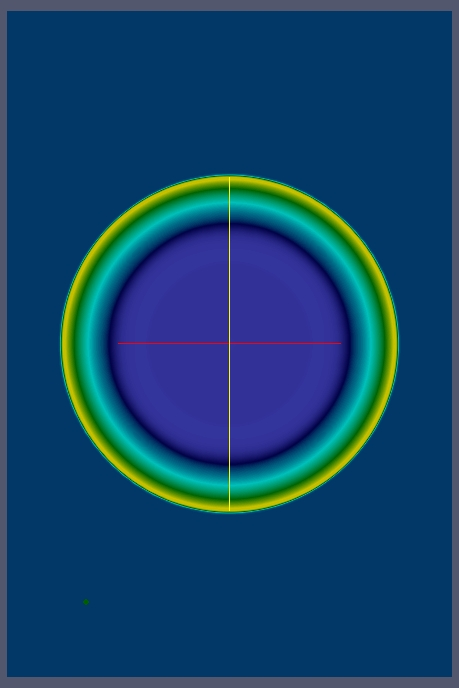
\includegraphics[width=0.5\textwidth]{fig/bw0020.jpg} & 
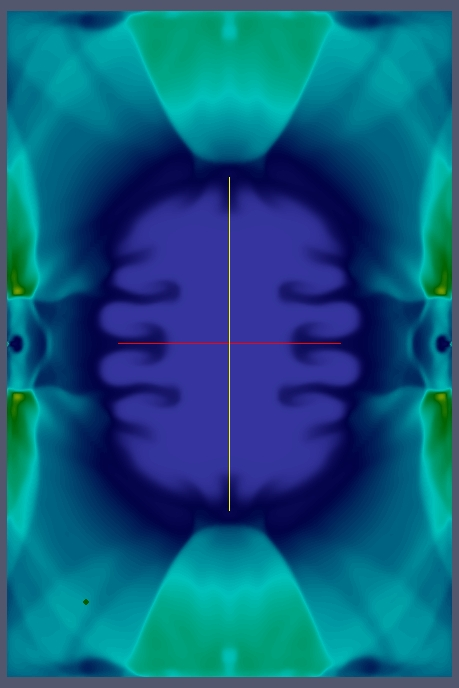
\includegraphics[width=0.5\textwidth]{fig/bw0175.jpg} 
\end{tabular}
\caption{Spherical blast waves at times: $t=0.2$ (left) and $t=1.75$ (right).  Simulation performed on a $400 \times 600$ grid of quadrilateral elements with code written for this dissertation available at: \protect\gitrepo.}
\label{fig:blast_waves}
\figSpace
\end{figure}

For the second case, a spherical blast wave is simulated on a rectangular domain with $L_y = 3L_x/2$ and periodic boundary conditions \citep{Zachary:1994,Balsara:1999,Londrillo:2000}.  The problem is initialized with a high pressure region corresponding to $r < 0.1$ where the gas pressure is two orders of magnitude greater than the background pressure.  A uniform density of $\rho = 1$ is used throughout the domain; the background gas pressure is $0.1$; the ratio of specific heats is $\gamma = 5/3$.

The density at times $t = 0.2$ and $t = 1.5$ is shown in the left and right panels of Figure~\ref{fig:blast_waves} respectively.  The blast wave is initially spherical as there are no effects due to grid alignment.  As the blast reaches the boundaries, complex interactions between linear and nonlinear waves are produced and solution remains symmetric across the $x$ and $y$ axis.  

%----------------------------------------------------------------
% Spherical Blast waves
%-----------------------------------------------------------------
\begin{figure}[htbp]\figSpace 
\begin{center}
\begin{tabular}{c}
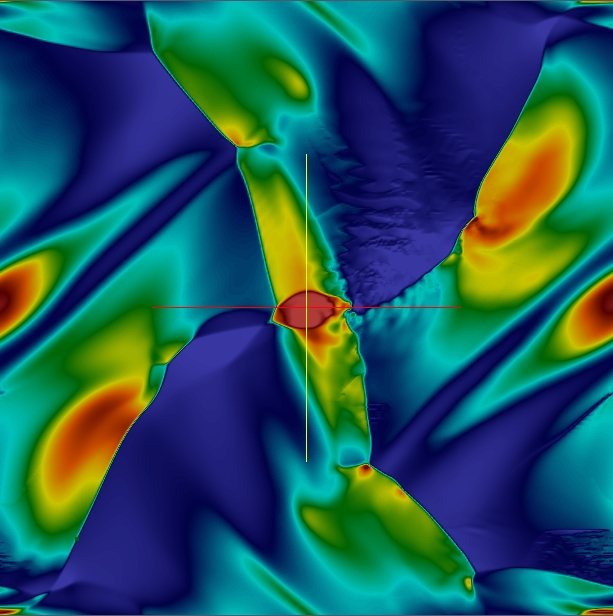
\includegraphics[width=0.5\textwidth]{fig/orszag_tang_010.jpg} \\
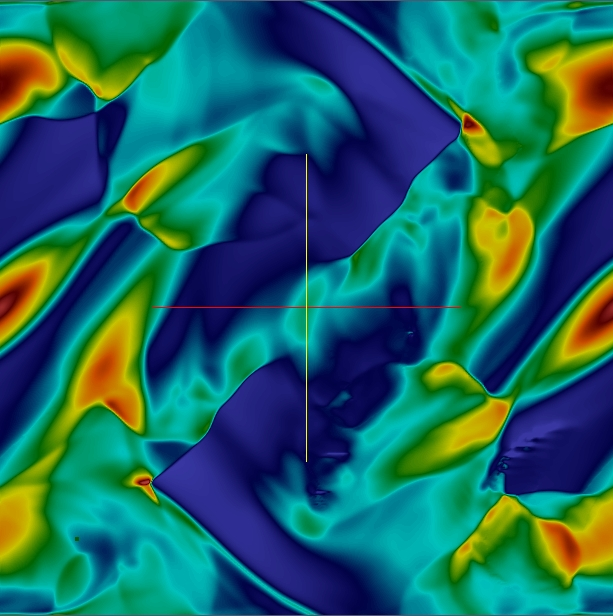
\includegraphics[width=0.5\textwidth]{fig/orszag_tang_015.jpg} 
\end{tabular}
\caption{Orszag-Tang vortex: $t=1.0$ (left) and $t=1.5$ (right).  Simulation performed on a $400 \times 400$ grid of quadrilateral elements with code written for this dissertation available at: \protect\gitrepo.}
\end{center}
\label{fig:orszag_tang}
\figSpace
\end{figure}

The Orszag-Tang vortex \citep{Orszag:1979} has been extensively studied and used for comparisons to previous results.  The simulation is performed on a square domain, $[0,1] \times [0,1]$, with periodic boundaries everywhere.  The density, $\rho = 25/(36\pi)$ and pressure, $5/(12\pi)$ are constant throughout the domain.  The initial velocities are $v_x = -\sin{(2\pi y)}$ and $v_y = \sin{(2\pi x)}$; the initial magnetic field is defined in terms of the magnetic vector potential, $A_z = B_0\left(\cos{(4\pi x)}/(4\pi) + \cos{(2\pi x)}/(2\pi)\right)$, where $B_0 = 1/\sqrt{4\pi}$; the ratio  of specific heats is $\gamma = 5/3$.  The solution at $t=1.0$ and $t=1.5$ is shown in Figure~\ref{fig:orszag-tang}.


%-----------------------------------------------------------------
% Performance results 
%-----------------------------------------------------------------
\begin{table}[htbp]\figSpace
\caption{Performance comparison of GPU and CPU (Ratio of  cells/sec.). }
\begin{tabular*}{\textwidth}{@{\extracolsep{\fill}} cccc}
\\ 
\hline 
\hline 
grid size & KH-Instability & Blast Waves & Orszag-Tang \\
\hline
$64\times64$ & 5 & 5 & 5 \\
$128\times128$ & 19 & 19 & 22 \\
$256\times256$ & 58 & 58 & 60 \\
$512\times512$ & 75 & 75 & 79 \\
$1024\times1024$ & 81 & 81 & 86 \\
\hline
\end{tabular*}
\label{tab:performance}
\figSpace
\end{table}

Performance comparisons between the GPU and CPU for the three test cases described above are listed in Table~\ref{tab:performance}.  The CPU has six physical cores and two logical cores per physical core, making 12 cores available with hyper-threading enabled.  Assuming near perfect scaling, running on the GPU is approximately seven times faster than running in parallel on the CPU.  A larger increase in performance of the GPU over the CPU is observed in the MHD test as compared to the HD tests.  The MHD equations are more complex than the HD equations and more calculations are required per time step.  The performance increase demonstrates the superior ability of the GPU to process many operations simultaneously.  

 The results indicate that the cost to performance ratio for a  GPUs such as NVIDIAs GTX Titan, which retails for about \$1000.00, is such that they are an ideal choice for shared memory processors, if the limited memory is managed properly.  The relatively large memory capacity of 6 GB on the GTX Titan is around $6.5\%$ of the 92 GB available on the Xeon E5.  For the equivalent memory of one Xeon E5, fifteen GPUs are required, costing nearly three times that of one Xeon E5.  In order for GPUs to be worth the investment, computations on the fly must be maximized and data storage minimized.  


%-----------------------------------------------------------------
% Timing Results Orszag-Tang
%-----------------------------------------------------------------
%% \begin{table}[htbp]\figSpace
%% \caption{Performance comparison of GPU and CPU Orszag-Tang results.}
%% \begin{tabular*}{\textwidth}{@{\extracolsep{\fill}} cccc}
%% \\ 
%% \hline 
%% \hline 
%% grid size & cells/second (GPU) & cells/second (CPU) & speed ratio \\
%% \hline
%% $64\times64$ & $4.1894\times10^6$ & $7.3955\times10^5$ & 5 \\
%% $128\times128$ & $1.6540\times10^7$ & $7.5060\times10^5$ & 22 \\
%% $256\times256$ & $4.4497\times10^7$ & $7.3155\times10^5$ & 60 \\
%% $512\times512$ & $6.3286\times10^7$ & $7.9437\times10^5$ & 79 \\
%% $1024\times1024$ & $7.2134\times10^7$ & $8.3354\times10^5$ & 86 \\
%% \hline
%% \end{tabular*}
%% \figSpace
%% \end{table}


